\documentclass{standalone}
\usepackage{tikz}
\usepackage{ctex,siunitx,ninecolors}
\setCJKmainfont{Noto Serif CJK SC}
\usepackage{tkz-euclide}
\usepackage{amsmath}
\usetikzlibrary{patterns, calc}
\usetikzlibrary {decorations.pathmorphing, decorations.pathreplacing, decorations.shapes}
\begin{document}
\small
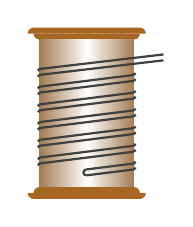
\begin{tikzpicture}[>=latex, scale=0.75]
  % \useasboundingbox(0.9,0)rectangle(5.1,5);
  \fill[brown5](-1,0)arc(180:90:0.1)--(0.9,0.1)arc(90:0:0.1)--cycle;
  \fill[brown5](-0.9,0)arc(-180:-90:0.1)--(0.8,-0.1)arc(-90:0:0.1)--cycle;
  \fill[left color=brown6!50!gray,right color=brown6!50!gray,middle color=white](-0.8,-0.1)rectangle(0.8,-2.6);
  \fill[brown5](-0.9,-2.7)arc(180:90:0.1)--(0.8,-2.6)arc(90:0:0.1)--cycle;
  \fill[brown5](-1,-2.7)arc(-180:-90:0.1)--(0.9,-2.8)arc(-90:0:0.1)--cycle;
  \foreach \y in {-0.9,-1.2,...,-2.3}
  {
    \draw[darkgray,thick](0.8,\y+0.1)--(-0.8,\y-0.1)arc(90:270:0.015);
    \draw[darkgray,thick](0.8,\y+0.1)arc(-90:90:0.015);
    \draw[darkgray,thick](0.8,\y+0.2)--(-0.8,\y)arc(90:270:0.015);
    \draw[darkgray,thick](0.8,\y+0.2)arc(-90:90:0.015);
  }
  \draw[darkgray,thick](1.3,-0.4531)--(-0.8,-0.7)arc(90:270:0.015);
  \draw[darkgray,thick](1.3,-0.3531)--(-0.8,-0.6)arc(90:270:0.015);
  \draw[darkgray,thick](0,-2.3)--(0.8,-2.2)arc(-90:90:0.015);
  \draw[darkgray,thick](0,-2.4)--(0.8,-2.30)arc(-90:90:0.015);
  \draw[darkgray,thick](0,-2.4)arc(-82.875:-262.875:0.0496)--(0,-2.3);
\end{tikzpicture}
\end{document}